
\begingroup
\frametitle{ Neuronale Netze: Black Box?}
\begin{frame}[plain]
	\centering
	
\uncover<1->{	\begin{tikzpicture}[scale=1, every node/.style={font=\small}]
		% Input Text
		\node at (-5.5, 2) {Input $x \in \mathbb{R}^n$};
		
		% Pfeil von Input zum Hut
		\draw[very thick, ->] (-3,2) -- (-1.8,2);
		
		% Magic Hat Image
		\node at (0, 2.6) {
\includegraphics[width=2.2cm]{BilderPräsentation/magic_hat.png}};
		\node at (0, 1.3) {\footnotesize Neural Network};
		
		% Pfeil von Hut zu Output
		\draw[very thick, ->] (1.4,2) -- (2.8,2);
		
		% Output Text
		\node at (5.2, 2) {Output $g(x)$};
	\end{tikzpicture}}
	
	\vspace{1.5em}
\uncover<2->{	\textbf{Frage:} Können neuronale Netze wirklich jede Funktion lernen?}

\end{frame}
\endgroup

\begingroup
\frametitle{ Universal Approximation Theorem}
\begin{frame}
	\centering
	\begin{tikzpicture}[baseline=(current bounding box.center)]

	% Zauberhut-Bild mittig
	\node (hat) at (-4.2, 0.2) {
\includegraphics[width=2.3cm]{BilderPräsentation/magic_hat.png}};
	\node[below=0.3em of hat] {\scriptsize \textit{Universal Approximation Theorem}};
	
	% Theorem-Box rechts daneben
		% Formelkasten rechts daneben
		\node[anchor=west] (box) at (-1.3, 0) {
			\begin{tcolorbox}[colback=blue!5!white,
				colframe=blue!70!black,
				boxrule=0.6pt,
				sharp corners,
				width=0.61\linewidth,
				halign=left]
				\small
				Für jede stetige Funktion \( f \in C([0,1]^n) \) und jedes \( \varepsilon > 0 \)
				existiert ein neuronales Netz \( g \) der Form
				\[
				g(x) = \sum_{j=1}^{m} w^{(2)}_j\, \sigma\big( x^\top w^{(1)}_j - b_j \big)
				\]
				sodass \( \|f - g\|_\infty < \varepsilon \).
			\end{tcolorbox}
		};
		
	\node[anchor=north west] at ([yshift=-0.8em]box.south west) {
		\begin{tcolorbox}[enhanced, sharp corners, boxrule=0pt, colback=white, width=0.7\linewidth, left=0pt, right=0pt, top=0pt, bottom=0pt]
		\end{tcolorbox}
	};

	\end{tikzpicture}
\vfill
{\tiny Quelle:G. Cybenko, “Approximation by superpositions of a sigmoidal function”, \textit{Mathematics of Control, Signals and Systems}, 1989~\cite{cybenko:hal-03753170}}
\end{frame}
\endgroup


\begingroup
\frametitle{Wie funktionieren neuronale Netze in der Praxis?}
\begin{frame}[plain]
\vfill
\begin{minipage}[c]{0.53\linewidth}
	\begin{itemize}
		\item Datengesteuerte, nichtlineare Funktionsapproximation
		\item Aufbau aus Layern \( f_1, f_2, \dots, f_L \)
		\item Lernen durch Backpropagation
		\item Architektur als Komposition:
	\[
	g(x) = f_L \circ f_{L-1} \circ \dots \circ f_1(x)
	\]
\end{itemize}
\end{minipage}
\hfill
\begin{minipage}[c]{0.44\linewidth}
	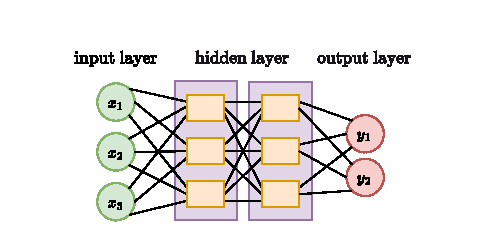
\includegraphics[width=0.95\linewidth]{BilderPräsentation/NN_ausgerichtet.drawio.pdf}
	\begin{itemize}\item []	{\scriptsize Schematische Darstellung eines neuronalen Netzwerks: Eingabe \(x_1, x_2, x_3\) wird durch eine Sequenz nichtlinearer Layer in Ausgaben \(y_1, y_2\) transformiert.} \end{itemize}

\end{minipage}
\vfill
\end{frame}
\endgroup

\section{Natural Language Processing}
\frame{\tableofcontents[currentsection]}

\begingroup
\frametitle{Definition: Language Encoder}

\begin{frame}
	\begin{block}{Language Encoder}
\small
Ein \textbf{Language Encoder} ist eine Abbildung
\[
h : \Sigma^* \rightarrow \mathbb{R}^D,
\]
die Texte \(x \in \Sigma^*\) aus einem Alphabet \(\Sigma\) auf Vektoren \(h(x)\) im Repräsentationsraum \(\mathbb{R}^D\) abbildet.

\vspace{0.3em}
Die Menge aller solcher Encoder ist \(\mathcal{E}_V := V^{\Sigma^*}\).

	\end{block}
\end{frame}

\endgroup


\begingroup
\frametitle{Sprachverarbeitung mit Encoder-Decoder-Modellen}
\begin{frame}
	\centering
	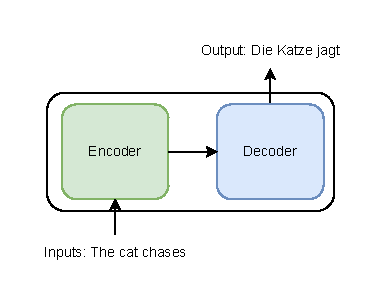
\includegraphics[width=0.4\linewidth]{BilderPräsentation/encoder_decoder.pdf}
	
	\begin{itemize}
		\item Encoder erzeugt eine Vektorrepräsentation aus dem Input-Text
		\item Decoder generiert daraus eine Zielsprache (z.\,B.\ Übersetzung)
		\item Modell lernt die Repräsentation durch Training auf großen Textdaten
	\end{itemize}
\end{frame}


\endgroup



